% !TEX program = xelatex
% spell-checker: disable
\documentclass{booklet_style}

%\usepackage[pagewise, mathlines]{lineno}

%\usepackage[draft]{todonotes}
% \usepackage[disable]{todonotes} % notes not showed

\sloppy
\frenchspacing

\usepackage[hyperref=true,
            backref=true,
            style=numeric-comp,
            sorting=none,
            maxnames=11,
            giveninits=false,
            url=false,
            isbn=false,
            defernumbers=true
            ]{biblatex}

\renewbibmacro{in:}{}
\AtEveryBibitem{%
    \clearlist{language}%
}

\addbibresource{sajat.bib}
\addbibresource{EMBL.bib}
\addbibresource{mouse.bib}

\DeclareRefcontext{journal}{labelprefix=J}

\DeclareBibliographyCategory{journal}
\addtocategory{journal}{balazs_real-time_2017,de_medeiros_light-sheet_2016,strnad_inverted_2016,hoyer_breaking_2016}

%\DeclareRefcontext{others}{labelprefix=J}

\DeclareBibliographyCategory{others}
\addtocategory{others}{jakus_genetic_2010,gyorffy_recurrenceonline:_2011,shi_combined_2014}


\DeclareRefcontext{conference}{labelprefix=C}
\DeclareBibliographyCategory{conference}
\addtocategory{conference}{balazs_gpu-based_2016,balazs_gpu-based_2016-1,balazs_gpu-based_2017}

\defbibheading{secbib}[\bibname]{
\section*{#1}
\markboth{#1}{#1}}


\def\b3d{B\textsuperscript{3}D}

\author{\href{mailto:balint.balazs@embl.de}{Balázs Bálint}}
\supervisor{Témavezető: \href{mailto:rozsabal@koki.hu}{Rózsa Balázs, \textit{M.D., Ph.D.}}}
\lab{\href{http://www.embl.de/}{European Molecular Biology Laboratory}}
\university{\href{http://www.ppke.hu/}{Pázmány Péter Katolikus Egyetem}}
\collegeordept{\href{http://www.itk.ppke.hu/}{Információs Technológiai és Bionikai Kar \\ Roska Tamás Műszaki és Természettudományi Doktori Iskola}}
\degreedate{\textit{A Ph.D. disszertáció tézisei} \\ Budapest, 2017}
\ppke{
\includegraphics[width=2cm]{figures/0_front/ITK_logo}}
\embl{
\includegraphics[width=2.5cm]{figures/0_front/EMBL_logo}}
\degree{PhD}

\title{Light-sheet mikroszkópia és valós idejű képfeldogozás új szemszögből}
%\date{2012 november}



\begin{document}

\graphicspath{{./figures/}}
%\begin{linenumbers}
\maketitle
%\pagenumbering{roman}

\clearpage{\thispagestyle{empty}\cleardoublepage}


\setcounter{page}{1}
\section{Bevezető}

A képalkotó eljárások, mint például a mikroszkópia az egyik legyakrabban használt eszközök az orvosi és biológiai kutatások során. Ennek az oka egyszerű: a puszta szem számára láthatatlan dolgok megjelenítése egy rendkívül hatásos módja annak, hogy betekintést kapjunk az ilyen dolgok belső működésébe. Az agyunk úgy fejlődött ki, hogy rengeteg külső információt dolgozzon fel, és ezek közül vitathatatlanul a látás a legjelentősebb.

Az optika egyik ágaként a mikroszkópia (görög erdet, mikrosz, ,,apró" és szkopein ,,figyel" szavakból) a fény és vizsgált minta interakcióinak megfigyelésén alapul. Hogy láthassuk ezeket az interakciókat, a mikroszkóp optikája felnagyítja a minta képét, ami detektálható és rögzíthető egy erre alkalmas berendezéssel. A legelső mikroszkópoknál, a 17. században, ez egyszerűen a szem volt, a felvételt pedig a megfigyelt képekről készült rajzok alkották \cite{hooke_micrographia:_1665}.

A mikroszkópia egy igazán multidiszciplináris tudományág: még a legegyszerűbb formájában, egy egyszerű lencsét használva, a fizika alapelveit kihasználva nyerhetünk mélyebb megértést a bilógiáról és a természetről. Manapság a mikroszkópia felöleli a legtöbb természettudomány eredményeit, kiegészítve különféle technológiia fejlesztésekkel. Ugyan továbbra is a fizika és a biológia adják a kulcsszerepet, a kémia (fluoreszcens molekulák), mérnöki tudmányok (automatizálás) és infromációs technológia (képfeldolgozás) eredményi közösen alkotják a modern mikroszkópia alapjait.

\section{Kihívások az élő minták háromdimenziós képalkotásában}


\subsubsection{Kihívások a képalkotásban}

Az élő mintákról történő képalkotás elengedhetetlen az embrionális fejlődés folyamatainak megértéséhez. Az ideális esetben a mikroszkóp képes lenne egy folyamatos, háromdimenziós, többszínű felvételt készíteni bármely biológiai folyamatról, a lehető legnagyobb felbontással. Sajnos azonban ez nem lehetséges; a biológia és fizika határai miatt kompromisszumra van szükség. A fény diffrakciós természete, a fluoreszcens jelölők véges élettartama és az élő minták fényérzékenysége miatt a mikroszkópiának alkalmazkodnia kell az aktuálisan megválaszolandó kérdéshez. Annak érdekében, hogy valóban hasznos felvételek készülhessenek, meg kell találni az egyensúlyt a jel-zaj viszony növelése és a térbeni és időbeni felbontás javítása közt, mindeközben szemmel tartva, hogy a maga a képalkotás ne legyen befolyással a vizsgálandó folyamatokra (\autoref{fig:tradeoffs}) \cite{laissue_assessing_2017}.

A light-sheet fluorescens mikroskópia (LSFM), másnéven egy-sík megvilágítású mikroszkópia (single plane illumination microscopy, SPIM) \cite{huisken_optical_2004} egy viszonylag új tagja azon technikák arzenáljának, melyek a fénymikroszkópián alapulnak. Nagy előnye, hogy különsen alkalmas élő minták hosszantartó vizsgálatára nagy térbeni és időbeni felbontással \cite{keller_quantitative_2008, huisken_selective_2009, weber_light_2011,tomer_shedding_2011}; továbbá könnyen adaptálható a vizsgálandó mintához, lehetővé téve számos különféle vizsgálatot, akár teljes szervek esetén \cite{dodt_ultramicroscopy:_2007}, "akár az egyes sejtek belsejében zajló folyamat \cite{chen_lattice_2014}."


Even though light-sheet microscopy offers intrinsic optical sectioning
To achieve isotropic 3D resolution, multiple views from different directions can be combined \cite{preibisch_efficient_2014}. This is most commonly achieved by embedding the sample in an aqueous gel which offers unrestricted view from multiple directions, and a stiff environment to position the sample \cite{krzic_multiview_2012}. Gel embedding, however is not always possible. Delicate samples, such as mouse embryos, require a very specific environment for proper development \cite{doherty_culture_2000}, which makes sample rotation impossible.





\begin{figure}[bht]
  \centering
  \begin{subfigure}[b]{0.49\textwidth}
    \raggedright
    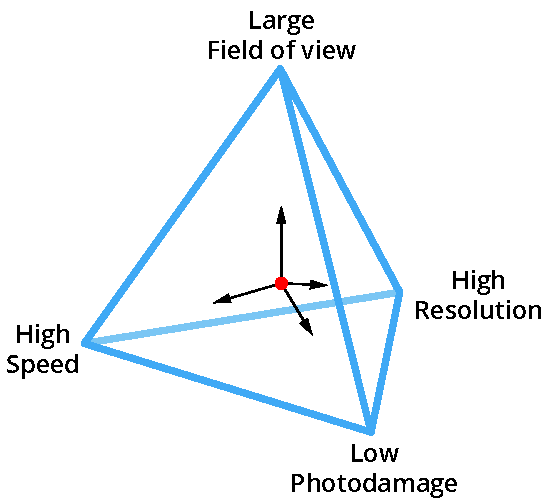
\includegraphics[width=0.9\textwidth]{1_spim/tradeoffs}
    \caption{}
    \label{fig:tradeoffs}
  \end{subfigure}
  \begin{subfigure}[b]{0.49\textwidth}
    \raggedleft
    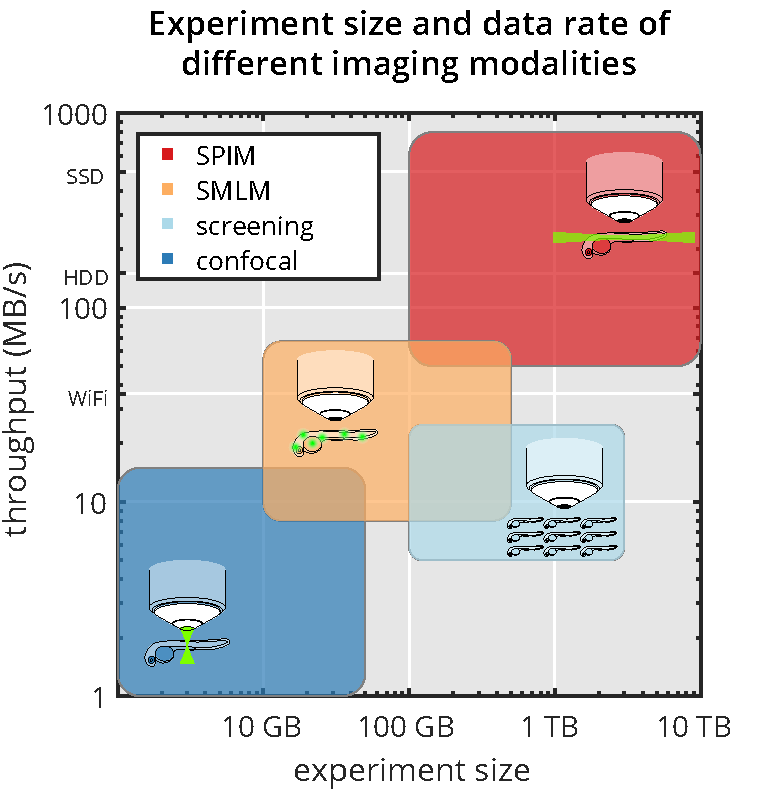
\includegraphics[width=0.9\textwidth]{4_gpu/comparison_with_pictograms}
    \caption{}
    \label{fig:sizes}
  \end{subfigure}
  \bcaption[Challenges in microscopy]{(a) Tradeoffs in fluorescence microscopy for live imaging. When optimizing the imaging conditions (red dot), a tradeoff has to be made between resolution, contrast, and imaging speed, while avoiding photodamage. Adapted from \cite{laissue_assessing_2017}.
  % Adapted from \cite{laissue_assessing_2017}.
  (b) Experiment sizes and data rate of different imaging modalities. Comparison of single-plane illumination microscopy (SPIM, red), high-content screening (light blue), single molecule localization microscopy (SMLM, orange) and confocal microscopy (blue) by typical experiment size and data production rate.
  % Also called the ``pyramid of frustration". When optimizing the imaging conditions (red dot), a tradeoff has to be made between resolution, contrast, and imaging speed, while avoiding photodamage. One can only be improved at the expense of the others due to the limited photon budget of the fluorescent molecules.
  }
  \label{fig:intro}
\end{figure}

% A selective-plane illumination microscope (SPIM) uses a light-sheet to illuminate only a thin section of the sample. This illumination plane is perpendicular to the imaging axis of the detection objective and coincides with the focal plane. This way, only the section in focus will be illuminated, thus providing much better signal to noise ratio compare to wide-field illumination. In case of conventional wide-field fluorescence microscopy, where the whole specimen is illuminated, out of focus light contributes to a significant background noise. 
% With selective-plane illumination, this problem is intrinsically solved, and it also provides a true sectioning capability. This makes SPIM especially suitable for 3D imaging.

\subsubsection{Kihívások a képfeldolgozásban}

When using any kind of microscopy in research, image processing is a crucial part of the workflow. This is especially true for light-sheet microscopy, since it is capable of imaging the same specimen for multiple days, producing immense amounts of data. A single overnight experiment of \textit{Drosophila} development (which is a very typical use-case for light-sheet microscopy) can produce multiple terabytes of data.

Apart from light-sheet microscopy, many other microscopy modalities are also suffering from this problem. Methods, such as high content screening \cite{carpenter_systematic_2004,echeverri_high-throughput_2006,pepperkok_high-throughput_2006}, where tens of thousands of different genotypes are imaged generating millions of images; and single molecule localization microscopy (SMLM) \cite{betzig_imaging_2006,hess_ultra-high_2006,rust_sub-diffraction-limit_2006}, where just a single plane of a sample is imaged hundreds of thousands of times to acquire super-resolved images.

Not only these methods are capable of generating data extremely fast, but with the sustained high data rate a single experiment can easily reach multiples of terabytes (\autoref{fig:sizes}). Handling this amount of data can quickly become the bottleneck for many discoveries, which is a more and more common issue in biological research \cite{wollman_high_2007,reynaud_guide_2015,perkel_struggle_2016}. 






% \section{Real-time image processing and compression}

% \begin{figure}[bt]
%   \centering
%   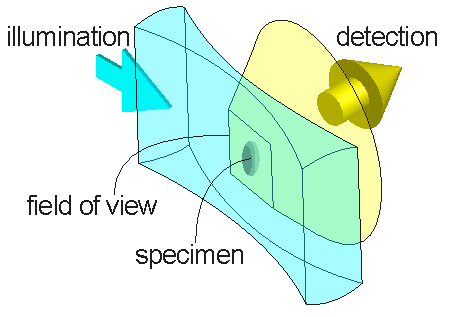
\includegraphics[width=0.6\textwidth]{spim_concept}
%   \bcaption[Basic concept of single-plane illumination microscopy]{The sample is illuminated from the side by laser light shaped to a light-sheet (blue). This illuminates the focal plane of the detection lens, that collects light in a wide-field mode (yellow). The image is recorded, and the sample is translated through the light-sheet to acquire an entire 3D stack.}
%   \label{fig:spim_concept}
% \end{figure}

\section{Új tudományos eredmények}

This work tackles the previously outlined challenges in light-sheet microscopy: high resolution live imaging of delicate samples, such as mouse embryos, and real-time image processing and compression of large light-sheet datasets.

  \paragraph{Tézis I.}\textit{Megterveztem es megépítettem egy light-sheet mikroszkópot, ami érzékeny minták nagy felbontású vizsgálatára alkalmas. A két darab, magas numerikus apertúrájú objektív 120 fokban történő elhelyezése, egy megdöntött light-sheettel kombinálva, izotróp 3D felbontású képalkotásra ad lehetőséget, miközben a fény begyűjtésének hatékonyságát kétszeresre növeli meg.}
  
    Kapcsolódó publikációk: \cite{de_medeiros_light-sheet_2016},\cite{strnad_inverted_2016}, \cite{hoyer_breaking_2016}

    A Dual Mouse-SPIM egy újszerű megközelítést képvisel a light-sheet mikroszkópiában. A 120 fokban elhelyezett magas numerikus apertúrájú objektívek nemcsak a felbontás javítását eredményezi a hagyományos 90 fokos elrendezéssel szemben, hanem a nagyobb detektálási szögnek köszönhetően a fény begyűjtése kétszer hatékonyabban történik. Ez legfőképpen fényérzékeny minták esetén, mint például egér embriók esetén lehet előnyös, mivel a fototoxikus hatások lecsökkenthetők, míg a kontraszt megmarad. Mindét objektív használható megvilágításra és detektálásra is, ami lehetővé teszi a forgatás nélküli többnézetes felvételt.

    A mikroszkóp részeként megterveztem egy egyedi nyalábosztó egységet, ami lehetővé teszi csupán egyetlen galvo-szkenner használatát a light-sheet generáláshoz mindkét objektív esetén. Továbbá egy olyan testreszabott detektálás-összeolvasztó egységet is megterveztem, ami lehetővé teszi egyetlen kamera használatát mindkét nézetből.

    Karakterizáltam a mikroszkóp optikai tulajdonságait, meghatározva a megvilágítási profilt és a pontátviteli függvényt (PSF).
    A \SI{95}{\micro m}-es látómező egy \SI{3,6}{\micro m} vastagságú light-sheettel van egyenletesen megvilágítva. A mintaként használt gömböcskék két irányból történő képalkotása \SI{314}{nm} laterális és \SI{496}{nm} axiális felbontást eredményezett. Ez egy 2,67-szeres javulás egyetlen lencse axiális felbontásához képest. Ezen kívül demonstráltam a  mikroszkóp képességét Drosophila embriókról és az egér zigótákról készült felvételekkel. 
    

    \begin{figure}
      \centering
      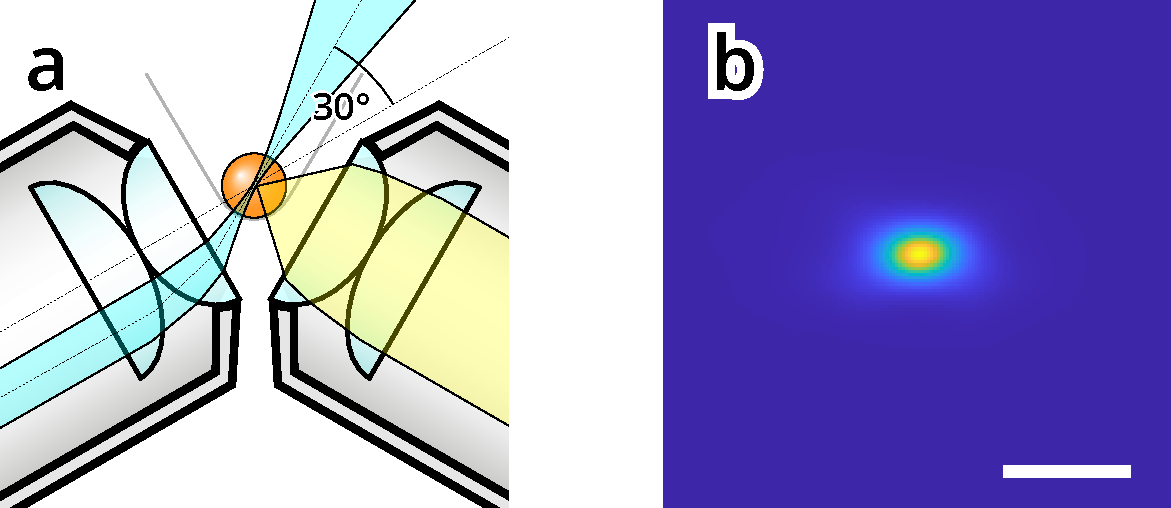
\includegraphics[width=0.9\textwidth]{2_DualMouse/120+psf}
      \bcaption[Dual Mouse-SPIM concept]{(a) Objective configuration. Both objectives can be used sequentially for both illumination and detection. (b) Combined PSF of the two views. Average of 12 fluorescent beads. Scale bar, \SI{1}{\micro m}.}
      \label{fig:DualMouse}
    \end{figure}


  \paragraph{Tézis II.} \textit{Kidolgoztam egy GPU-alapú képfeldolgozási pipeline-t többnézetes light-sheet mikroszkópiára, amely lehetővé teszi a szemközti nézetek valós időbeni összeolvasztását.}

    Kapcsolódó publikációk: \cite{balazs_gpu-based_2016}, \cite{balazs_gpu-based_2016-1}, \cite{balazs_gpu-based_2017}

    Kidolgoztam egy GPU-alapú képfeldolgozási pipeline-t, mely közvetlenül integrálható a LabVIEW alapú univerzális mikroszkóp vezérlő rendszerünkbe. A pipeline jelenleg lehetővé teszi a háttér levonását és a háttér maszkolását, továbbá képes az azonos sík szemközti nézeteinek azonnali összeolvasztására. Megmutattam, hogy lehetséges a szemközti nézetek regisztrálásának 3D problémáját 2D problémára redukálni, anélkül, hogy ez negatív hatással lenne a képminőségre és a felbontásra. Ez jelentősen lecsökkenti a szükséges számítási kapacitást és lehetővé teszi a CUDA textúrák alkalmazását és a valós időbeni összeolvasztást. Ennek a megoldásnak a feldolgozási sebessége 138 fps, ami 18.3-szoros növekedés az egyszálú CPU verzióhoz képest.


    \begin{figure}
      \centering
      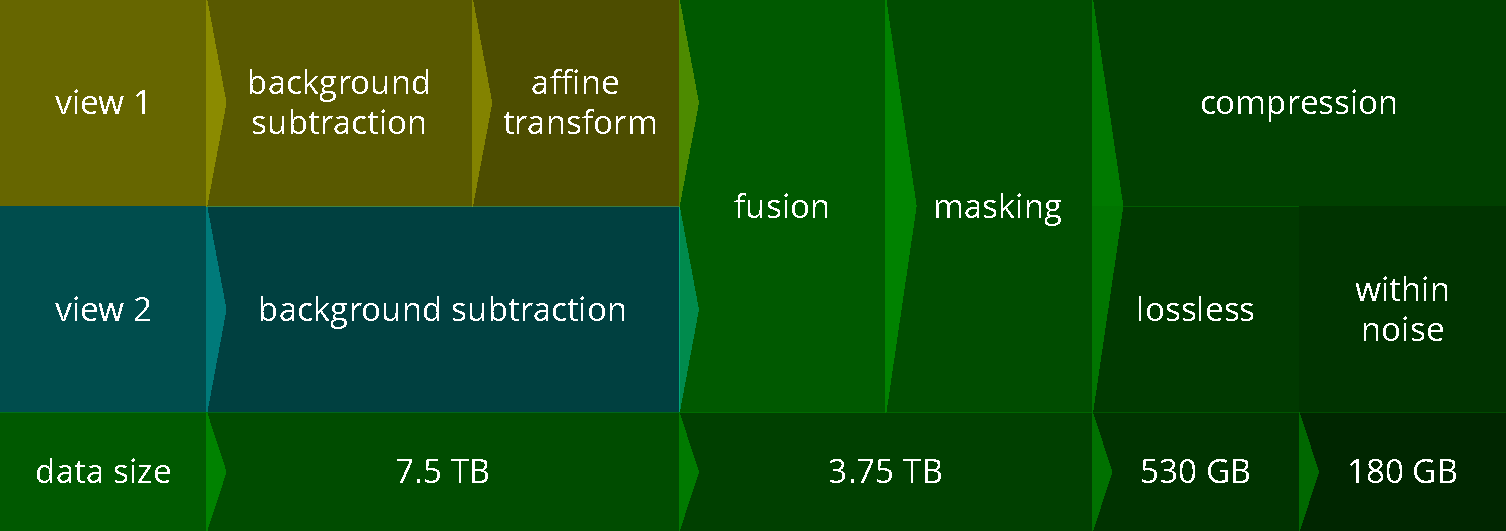
\includegraphics[width=\textwidth]{4_gpu/pipeline}
      \bcaption[Real-time image processing pipeline for multi-view light-sheet microscopy]{}
      \label{fig:pipeline}
    \end{figure}
    

  \paragraph{Tézis III.} \textit{Kifejlesztettem egy képtömörítési algoritmust, ami lehetővé teszi a fénymikroszkópokkal nyert képek zaj-függő veszteséges tömörítését és akár százszoros tömörítési arányt is elérhet, megőrizve a későbbi adatfeldolgozó lépések eredményeit. A gyors CUDA implementáció lehetővé teszi a nagysebességű kamerák képeinek valós idejű tömörítését.}

    Kapcsolódó publikációk: \cite{balazs_real-time_2017}, \cite{balazs_gpu-based_2016}, \cite{balazs_gpu-based_2016-1}, \cite{balazs_gpu-based_2017}
    
    % \b3d is an efficient, GPU-based image compression library allowing losslaess and noise dependent lossy compression of microscopy images.
    Mivel a számos különféle nagyebességű mikroszkópia technikák hatalmas mennyiségű adatot generálnak, kísérletenként akár terabájtokat elérve, a képtömörítés kiemelt szerepet kap ilyen adathalmazok esetén. A jelenleg használt, mikroszkópos képekkel kompatibilis képtömörítési eljárások nem képesek a modern sCMOS kamerák nagy adatsebességével megküzdeni ($\sim \SI{800}{MB/s}$).

    Kifejlesztettem a \b3d nevű GPU-alapú párhuzamos képtömörítő algoritmust, amely képes \SI{1}{GB/s} feletti átviteli sebességre, lehetővé téve a valós idejű képtömörítést. A méret további csökkentése érdekében kidolgoztam egy zajfüggő veszteséges tömörítési eljárást, amely determinusztikus módon módosítja az adatokat. A pixelenkénti megengedett eltérés a kép zajszintjéhez képest választható, figyelembe véve a sörétzaj (shot noise) és a kamera kiolvasási zaj mértékét. A pixel prediktálásnak köszönhetően a szubjektív képminőség magasabb, mint más eljárások esetén, ahol egyszerűen a képek négyzetgyökének kvantálása történik.
  


  \paragraph{Tézis IV.} \textit{Megmutattam, hogy a zajszinten belüli tömörítés nem befolyásolja szignifikánsan a leggyakrabban használt képfeldolgozási feladatok eredményeit és a tömörítési arány 3,32-szeres átlagos javulását eredményezi a veszteségmentes tömörítéshez képest.}
  
    Kapcsolódó publikációk: \cite{balazs_real-time_2017}, \cite{balazs_gpu-based_2016}, \cite{balazs_gpu-based_2016-1}, \cite{balazs_gpu-based_2017}
    
    Mivel az adatok integritása elengedhetetlen a megfelelő következtetések levonása érdekében, ezért a veszteséges tömörítés használata ellentmodnásos lehet.
    Megmutattam, hogy a \b3d zajszinten belüli módja (within noise level, WNL) nem befolyásolja szignifikánsan a leggyakrabban használt képfeldolgozási feladatok eredményét.
    
    Light-sheet mikroszkópos adatokra megmutattam, hogy a WNL tömörítés kisebb eltérést okoz a képben, mint a sörétzaj (shot noise). A felvételek szegmentálása esetén a szegmentált régiók átfedése \textit{Drosophila} embrió sejtmagokra 99,6\%, míg \textit{Phallusia} embriók membránjára 94,5\%. A tömörítési arány a két felvételre 19,3-szoros, illetve 40,01-szeres volt.
    
    \begin{figure}
      \centering
      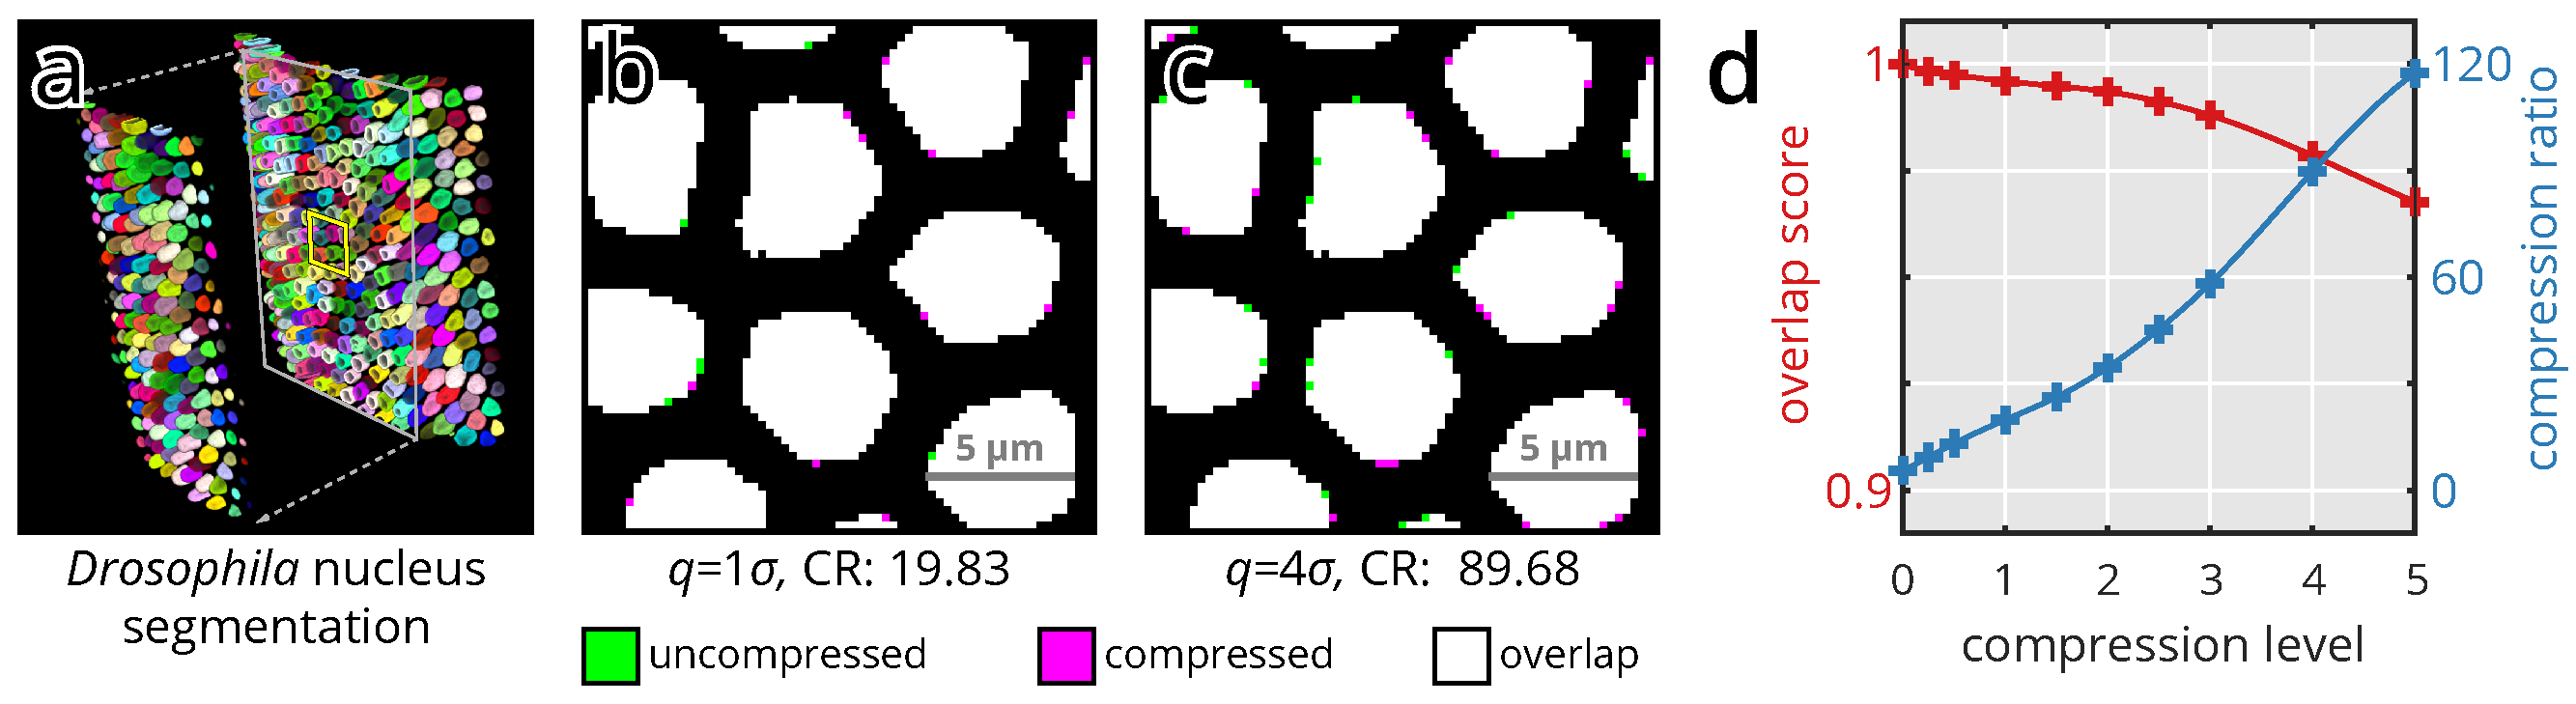
\includegraphics[page=1,width=\textwidth]{4_gpu/LLvsB3D}
      \bcaption[Influence of noise dependent lossy compression on 3D nucleus segmentation]{A \textit{Drosophila melanogaster} embryo expressing H2Av-mCherry nuclear marker was imaged in MuVi-SPIM \cite{krzic_multiview_2012}, and 3D nucleus segmentation was performed. (\textbf{a}). To visualize segmentation mismatch, the results of the uncompressed (green) and compressed (magenta) datasets are overlaid in a single image (\textbf{b}, \textbf{c}; overlap in white). For all compression levels the segmentation overlap score was calculated and is plotted in (\textbf{d}) along with the achieved compression ratios.}
      \label{fig:wnlDroso}
    \end{figure}

    Lokalizációs mikroszkóp adatokra megmuttam, hogy a WNL tömörítés mindössze 4\%-kal növeli a lokolizációs hibát, míg az átlagos tömörítási ráta 1,44-ről (veszteségmentes) 4,96-ra emelkedik. Megmutattam továbbá, hogy a lokalizációs hiba változása nem függ az felvételek jel-zaj viszonyától.

    


\section{Lehetséges alaklmazások}
Mind a Dual Mouse-SPIM mikroszkópnak, mind a GPU-alapú képfeldolgozásnak közvetlen alkalmazási lehetőségei vannak az embrionális fejlődés vizsgalatában. Több potenciális együttműködő fejezte ki érdeklődését a Dual Mouse-SPIM használata iránt az egérembrió fejlődésének vizsgálatához. A Hiiragi
csoport, akik a pre- es posztimplantációs fázis szimmetriatörő eseményeire összpontosítanak, szeretnék kipróbálni ezt az elrendezést a nagyobb minták több irányból történő képalkotására, ami a jelenleg használt mikroszkópjukkal nem működik es lehetőseget adhat eddig ismeretlen mechanizmusok feltárasára. Az Ellenberg csoport a kromoszóma szegregáció mechanizmusait vizsgálja az embrionális fejlődés első néhány osztódási fázisában. A nagyobb axiális felbontás lehetőséget ad minden egyes kromoszóma követésére az osztódási folyamat során, ami eddig nem volt lehetséges az axiális felbontás hiányosságai miatt.

A GPU-alapú képfeldolgozási pipeline-t, főképp a szemközti nézetek 2D fúzióját már most is használjuk laborunk nagyteljesítményű mikroszkopján, a MuVi-SPIM- en. A két szemközti objektív nézeteinek összeolvasztása a képalkotás közben nemcsak jelentős tárhely megtakarítást eredményez, de az adatelemzést is szignifikánsan felgyorsítja.

A \b3d képtömörítési algoritmus először light-sheet mikroszkópia kihívásaira fókuszálva lett megtervezve, de sokkal széleskörűbb felhasználási lehetőséget nyújt. Bármilyen nagy teljesítményű, high-throughput fénymikroszkópián alapuló vizsgálat profitálhat a zajszinten belüli tömörítési eljárásnak köszönhető jelentős adatcsökkenés adta előnyökből. Mivel a tömörítés a képalkotás alatt azonnal kivetelezhető, nemcsak a tárolási feltételek, de a szükséges sévszélesség is lecsökken, ami szükségtelenné teszi a nagyteljesítményű RAID tömbök hazsnálatát és 10 Gbit-es hálózat kiépítését tovább csökkentve a költségeket. A hasonlóan gyors kitömörítési sebességnek köszönhetően az
adatbeolvasás is gyorsabb lesz, amiből a böngészési és 3D adatmegjelenítési alkalmazások profitálhatnak. Néhany cég már érdeklődését fejezte ki a tömörítés iránt, többek között a Bitplane AG (3D adatelemzés és megjelenítés), Luxendo GmbH (light-sheet mikroszkópia) es Hamamatsu Photonics K.K. (kamera es szenzor gyártás).




% \cleardoublepage
% \section*{References}

\newrefcontext{journal}
\printbibliography[category=journal, title={A szerző közleményei a témában}, heading=secbib]
\markboth{\MakeUppercase{References}}{}

%\newrefcontext{others}
\nocite{jakus_genetic_2010,gyorffy_recurrenceonline:_2011,shi_combined_2014}
\printbibliography[category=others, title={A szerző további közleményei}, heading=secbib, resetnumbers=5]
\markboth{\MakeUppercase{References}}{}

\newrefcontext{conference}
\printbibliography[category=conference, title={A szerző konferencia előadásai}, heading=secbib]
\markboth{\MakeUppercase{References}}{}

\newrefcontext
\printbibliography[notcategory=journal,notcategory=conference,notcategory=others, resetnumbers=true, title={Refernciák}, heading=secbib]
\markboth{\MakeUppercase{References}}{}


%\end{linenumbers}
\end{document}